\section*{CHAPTER 2: BACKGROUND}
\addcontentsline{toc}{section}{\numberline{}CHAPTER 2: BACKGROUND}
\setcounter{section}{2}
\setcounter{subsection}{0}
\setcounter{figure}{0}
\setcounter{table}{0}

\subsection{OFDM Basics}

In digital communications, information is expressed in the form of bits. The term symbol refers to a collection, in various sizes, of bits [6]. OFDM data are generated by taking symbols in the spectral space using M-PSK, QAM, etc, and convert the spectra to time domain by taking the Inverse Discrete Fourier Transform (IDFT). Since Inverse Fast Fourier Transform (IFFT) is more cost effective to implement, it is usually used instead [3]. Once the OFDM data are modulated to time signal, all carriers transmit in parallel to fully occupy the available frequency bandwidth [7].During modulation, OFDM symbols are typically divided into frames, so that the data will be modulated frame by frame in order for the received signal be in sync with the receiver. Long symbol periods diminish the probability of having inter-symbol interference, but could not eliminate it. To make ISI nearly eliminated, a cyclic extension (or cyclic prefix) is added to each symbol period. An exact copy of a fraction of the cycle, typically 25\% of the cycle, taken from the end is added to the front. This allows the demodulator to capture the symbol period with an uncertainty of up to the length of a cyclic extension and still obtain the correct information for the entire symbol period.

\begin{figure}[ht]
    \centering
    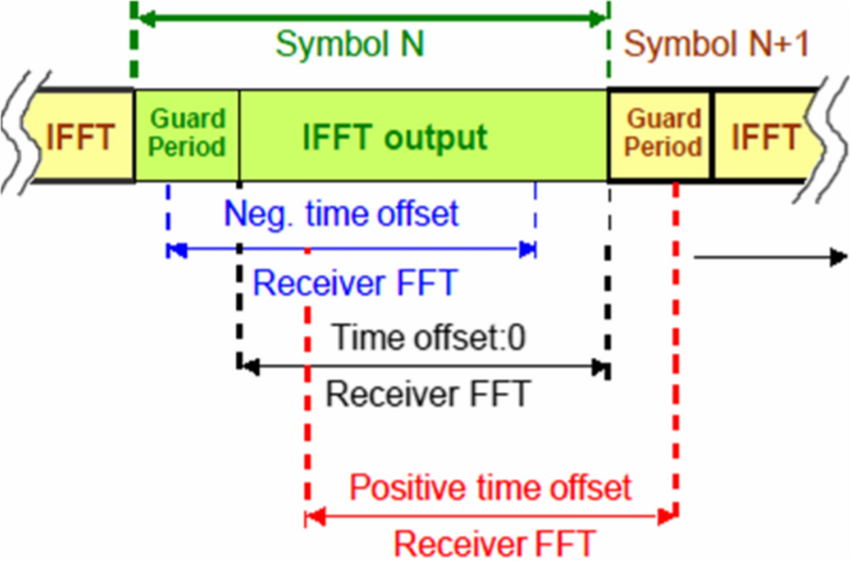
\includegraphics[width=0.5\textwidth]{Figures/Cyclic-extension-tolerance.png}
    \caption{\bfseries\centering\fontsize{13pt}{0pt}\selectfont Cyclic-extension-tolerance}
    \label{Cyclic-extension-tolerance}
\end{figure}

As shown in Figure \ref{Cyclic-extension-tolerance} [8], a guard period, another name for the cyclic extension, is the amount of uncertainty allowed for the receiver to capture the starting point of a symbol period, such that the result of FFT still has the correct information. In Figure 2 [9], a comparison between a precisely detected symbol period and a delayed detection illustrates the effectiveness of the cyclic extension.

\begin{figure}[ht]
    \centering
    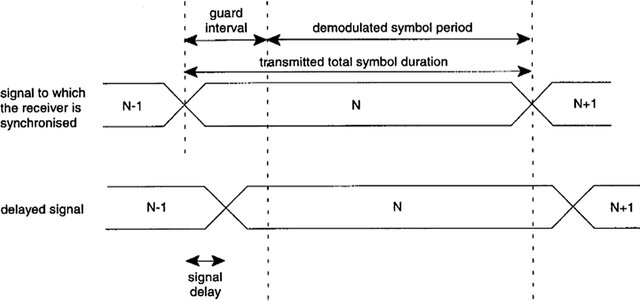
\includegraphics[width=\textwidth]{Figures/Effectiveness-of-cyclic-extension.jpg}
    \caption{\bfseries\centering\fontsize{13pt}{0pt}\selectfont Effectiveness-of-cyclic-extension}
    \label{Effectiveness-of-cyclic-extension}
\end{figure}

\subsection{OFDM Parameters and Characteristics}

The number of carriers in an OFDM system is not only limited by the
available spectral bandwidth, but also by the IFFT size, which is determined by the complexity of the system [10]. The more complex (also more costly) the OFDM system is, the higher
IFFT size it has; thus a higher number of carriers can be used, and higher data